\section{Pulsed Laser Deposition}
Thin film research is essential in science and 
technology and has led to countless inventions of electronic semiconductor devices.
Therefore, it is crucial to have a reliable and precise way to fabricate thin films. 
One method, which is not only reliable but also flexible and comparatively inexpensive,
is \ac{pld}. 
For this reason, the following sections aim to present the \ac{pld} structure and its 
working principles.
This discussion summarizes the work of \citeauthor{lorenz} \cite{lorenz}.

\subsection{PLD Explained in Steps}
A basic \ac{pld} setup is depicted in \cref{fig:pld_chamber}.
The process begins with a bulk material that serves as a material source for the thin 
film.
This source, called target, is installed into a vacuum chamber along with a 
substrate that serves as the foundation and growth template of the film.
For this lab course, a \ce{ZnO} target and a c-sapphire substrate was used.
A high-power pulsed laser beam in the ultraviolet spectral range is focused through a 
lens and directed through a window into the vacuum chamber, where it hits the target. 
During every laser pulse, the target material begins to ablate and evaporate. 
The evaporated material interacts with the laser photons as well and thus excites into a 
plasma. 
This plasma is directed towards the substrate, where it condenses.
After each pulse, some material is added and after a fixed number of pulses,
a thin film is deposited on the substrate. 

The laser-target interaction is a complex and nonequilibrium process and therefore
hard to model analytically.
Laser photons are absorbed by the target material and interact with the electronic 
system.
Due to electron-phonon interaction, energy of the electrons is converted 
into thermal, chemical and mechanical energy.
This leads to ablation and evaporation of the material.
The ejected species expand into vacuum, interact with the laser and form a plasma
plume. 
This plume consists of electrons, atoms, ions, molecules and clusters and is directed 
towards the substrate.

\ac{pld} runs inside a vacuum chamber under ultrahigh vacuum or under a controlled 
background gas pressure.
The background gas can be chosen, oxygen, nitrogen or argon are common candidates.
The substrate is normally heated using a resistive or laser heater.

 A \ac{pld} setup offers a very flexible system for investigating thin film materials.
It is applicable for a large material library, including oxides, nitrides and even
metals. 
For most materials it also ensures stoichiometric transfer from the target to the film.

\subsection{Design of a \ac{pld} System}
In this section, the structure of a \ac{pld} system shall be discussed.
\ac{pld} is a \ac{pvd} technique and thus characterized by a process in which the target
material transitions from a condensed phase to a vapor phase and then back to a thin 
film condensed phase on a substrate.
The evaporation process is accomplished by pulsed laser rays hitting the target inside
a vacuum chamber. 
Therefore, the laser and the chamber are  two main components that will be
explained in detail.

\subsubsection{Laser}
The most useful wavelengths for laser-induced ablation are in the range between
\qtyrange{200}{400}{\nano \meter}. 
In this region, most materials have a strong absorption and therefore a reduced 
penetration depth into the target. 
With that, thinner layers can be ablated, which generally increases thin film quality.
An adjustable lens should be installed into the beam path to focus the laser beam onto 
the target with a known spot size.

Commercial lasers in this spectral range are available and technically sophisticated.
Two commonly used laser architectures for \ac{pld} are Nd:YAG and excimer lasers.

\textbf{Nd:YAG Lasers}
are solid-state systems with an yttrium aluminum garnet (\ce{Y3AlO12}) host
crystal.
This crystal is doped with neodymium ion ($\ce{Nd^{{3+}}}$) impurities that serve as an
active medium.
The neodymium ions inside the YAG crystal are excited by flashlamps and can 
relax into energetically lower states by emission of \qty{1064}{\nano\meter} photons. 
The YAG crystal itself is not participating in photon emission.
Using a nonlinear crystal, the wavelength can be converted to \qty{266}{\nano\meter} 
radiation, though this process significantly reduces the intensity.

\textbf{Excimer Lasers} are gas lasers that emit photons directly in the ultraviolet 
spectral range.
The most common type is the krypton fluoride (\ce{KrF}) laser, which is used as 
a representative example. 
A gas mixture of krypton and flouride is pumped into the gas chamber of the laser.
This molecular gain medium has a metastable upper electronic state (excimer) 
and a repulsive ground state.
Through electric discharge, the constituents create excited species 
\cref{eq:excited_species} that can react to excimer molecules \cref{eq:excimer_formation}.
These molecules can relax by induced emission and emit photons \cref{eq:excimer decay}.
Due to the repulsive ground state, the ground state molecule is not stable and
dissociates into its components \cref{eq:dissociation}.

The formation of excimer molecules is complex and consists of several steps.
Only the most important reactions are listed below:
\begin{align}
	\label{eq:excited_species}
	\begin{split}
		\ce{Kr + e- &-> Kr+, Kr^*, Kr_2^+} \\
		\ce{F2 + e- &-> F + F-}
	\end{split}\\
	\noalign{\vskip 0.1cm}
	\label{eq:excimer_formation}
	\begin{split}
		\ce{Kr+ + F- + X &-> KrF^* + X} \\
		\ce{Kr_2^+ + F- &-> KrF^* + Kr} \\
		\ce{Kr^* + F2 &-> KrF^* + Kr} 
	\end{split} \\
	\noalign{\vskip 0.1cm}
	\label{eq:excimer decay}
	\begin{split}
		\ce{KrF^* &-> KrF + h\nu}
	\end{split} \\
	\noalign{\vskip 0.1cm}
	\label{eq:dissociation}
	\begin{split}
		\ce{KrF &-> Kr + F_2}
	\end{split}
\end{align}
In the preceded equations, $\mathrm{X}$ is a third body that is needed for the reaction 
to occur and stabilize the excimer. 
This can be another noble gas like argon or neon.

\begin{figure}[h!]
	\centering
	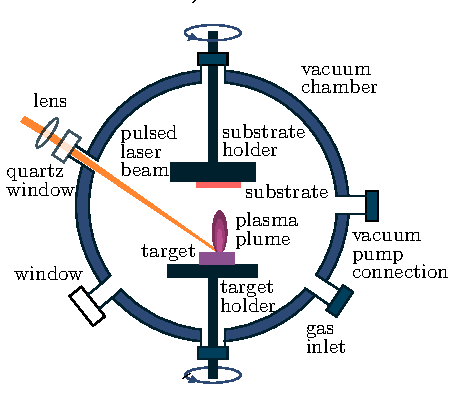
\includegraphics{../assets/pld_chamber}
	\caption{Schematic design of a \ac{pld} chamber. \imcitetwo{peter}}
	\label{fig:pld_chamber}
\end{figure}

\subsubsection{Vacuum Chamber}
A possible configuration of a \ac{pld} vacuum chamber is shown in 
\cref{fig:pld_chamber}.
The chamber is equipped with a quartz window, used as a laser beam entrance.
Viewport windows are beneficial for maintenance and monitoring and should
be installed.
These windows should be kept clean to ensure a high transmission of the laser beam
as well as a clear view into the chamber.

Vacuum pump connections and gas inlets are integrated into the chamber
to control a defined vacuum or atmosphere.
The vacuum pump operates at a constant rotational speed while the 
gas inlet valves handle pressure regulation. 

The mounted substrate holder offers various clamps for different substrate sizes.
Usually, a resistive or laser heating system is installed near the substrate holder to
manipulate the substrates temperature and thus the quality of the deposited thin film.
To achieve a more even temperature distribution, the substrate holder is able to rotate.

Towards the substrate holder, a target holder is installed.
This holder is able to rotate and translate as well.
Advanced systems have a target carousel, that can hold multiple targets and can be
rotated to select the desired one.

\subsection{Detailed Working Principle Analysis}
The working principle of a \ac{pld} system can be divided into three main steps, with
each step explained in detail in the following sections:
\begin{itemize}
	\item formation and composition of the laser plasma
	\item expansion of the plasma
	\item nucleation and growth of the film.
\end{itemize}

\subsubsection{Formation and Composition of the Laser Plasma}
Using an adjustable lens, the laser beam is focused onto the target 
with a power density in order of \qty{e8}{\watt\per\centi\meter\squared}.
This density is far above the materials thermal evaporation threshold that is usually 
around \qty{e7}{\watt\per\centi\meter\squared}.
As a result, the target material starts to ablate.

This ablation process is complex and nonequilibrium due to the discontinuous nature 
of the laser pulses but can be categorized in different mechanisms. 
The most common one is thermal ablation by absorption of the laser photons:
The laser photons are absorbed by the target material.
Due to their high energy, the target material ionizes and 
free electrons are generated.
Those electrons begin to oscillate as a response to the electromagnetic field 
and can collide with the atoms of the bulk material,
thus transferring energy to the lattice of the target material.
Electromagnetic energy is converted into thermal and chemical energy.
The material is heated up and begins to evaporate.

Apart from thermal ablation, nonthermal, photoinduced electronic sputtering can occur.
This mechanism is based on the direct interaction of the laser photons with the 
electronic system.
Due to electron excitation, chemical bonds can break, resulting in the ejection of
atoms or molecules from the target surface, without any significant temperature change. 

Droplets and flakes can be expelled from the target towards the substrate as a result
of plasma recoil pressure and thermal shocks. 
This leads to a reduction of thin film quality.

The target surface is altered during the ablation process, which results in target 
erosion.
This leads to a deviation of the surface normal, therefore changing the plasma 
plume's direction.
In order to ensure a uniform material removal, the target is rotated and translated.

\subsubsection{Expansion of the Plasma}

\begin{figure}
	\centering
	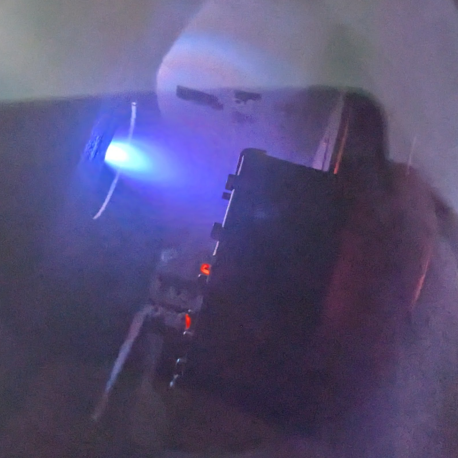
\includegraphics[width=0.6\columnwidth]{../assets/plume.pdf}
	\caption{Plasma plume in the PLD chamber used in the Leipzig 
	semiconductor research group.}
	\label{fig:plume}
\end{figure}

After the material is evaporated, it starts to interact with the laser photons too.
As a result, the material is excited and ionized and a plasma plume arises, see 
\cref{fig:plume}.
Due to Coulomb interaction and recoil from the target surface, 
the plasma expands perpendicular to the target's surface.

The spatial dependence of the plume depends strongly on the background gas pressure.
At a low background pressures around \qty{e-4}{\milli \bar} or lower, the plume is
narrow, and its constituents have a high velocity.
Only a few scattering events occur.

At intermediate pressures, between \qtyrange{e-3}{e-2}{\milli \bar},
 a splitting of high energetic from less energetic species can be observed.
In high-pressure regions with a background pressure of \qty{e-1}{\milli \bar} or 
higher, the expansion of the plasma is diffusion-like.
The plasma plume is wider and the velocity of the species is
reduced further.

The most important implication of increased background pressure is the slowdown of 
the energetic species in the plasma plume. 
A study demonstrated that the maximum kinetic energy of the constituents
with a laser fluence of \qty{2}{\joule \per \centi \meter \squared} at a background 
pressure of \qty{e-2}{\milli \bar} was approximately \qty{30}{\kilo \electronvolt}, 
whereas at \qty{e-1}{\milli \bar}, it was reduced to around 
\qty{4}{\kilo \electronvolt} \cite{xu2014}.

\begin{figure}
	\centering
	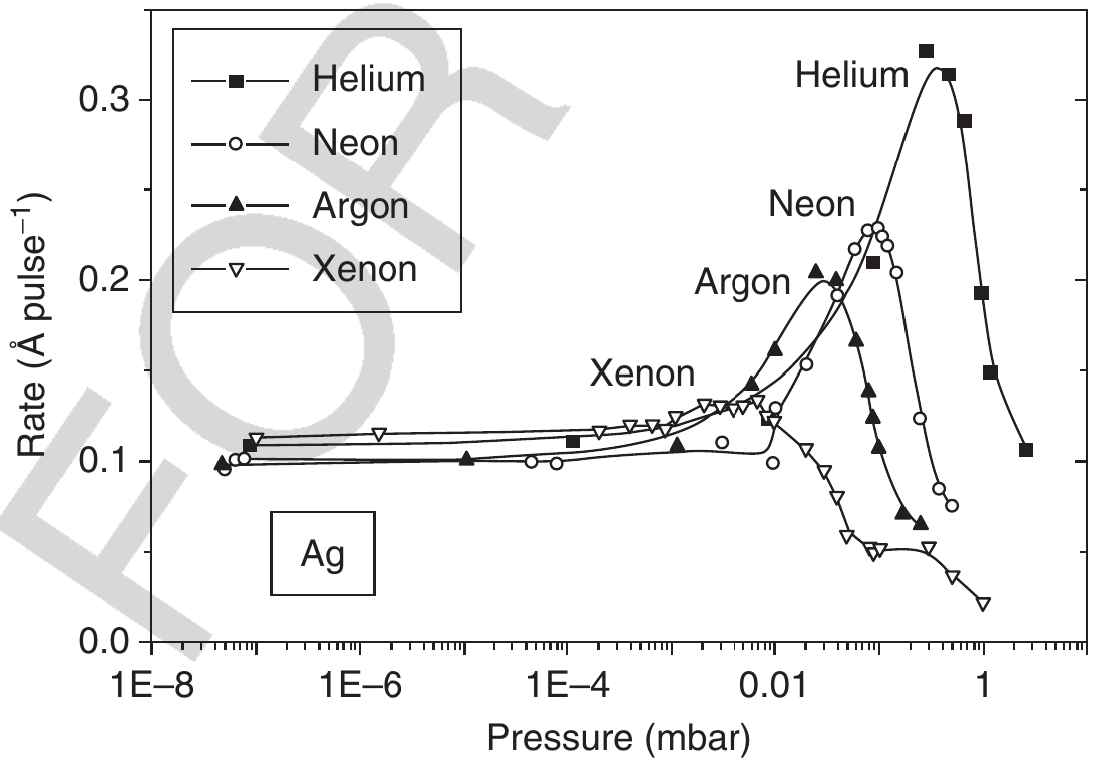
\includegraphics[width=0.98\columnwidth]{../assets/deposition_rate.png}
	\caption{Deposition rate as a function of background pressure for helium, neon, 
	argon and xenon background gases. \imcite{lorenz}}
	\label{fig:pld_plasma}
\end{figure}

The deposition rate, defined as the film thickness difference per laser pulse, is also 
influenced by the background pressure.
In \cref{fig:pld_plasma}, the deposition rate is shown as a function of the background
pressure for different background gases.
It can be seen that the deposition rate for low background pressures is low.
This is due to the high constituent velocity, which leads to resputtering of the
deposited material.
At higher background pressures, the particle velocity is reduced and the deposition
rate increases.
For even higher pressures, the deposition rate decreases again 
as a result of the slower and widespread plasma plume.

Background gas pressure can also lead to a change the stoichiometry of the deposited 
film.
Especially oxygen concentration in oxide films is strongly influenced by the
background pressure.

\subsubsection{Nucleation and Growth of the Film.}
The plasma plume is directed towards the substrate, where it condenses on 
the substrate surface and transforms again into solid state.
A nucleation process starts, resulting in thin film growth. 
This step is the most essential for thin film crystal quality.

High-energy species from the plasma plume bombard the substrate.
This can damage the substrate's crystal structure as well as sputtering off 
surface atoms.
Sputtered substrate particles together with plasma's constituents form a near-surface 
collision region that serves as a condensation nucleus. 
Supersaturation occurs on the substrate during the laser pulse, which leads to a
large nucleation density on the substrate surface.
As a result, other species from the plasma plume append on the condensation nuclei and
the thin film starts to grow.
The growth of the thin film can be divided into three different modes:

\textbf{Layer-by-Layer Growth} is a common growth mode, where monoatomic islands 
emerge until a critical density is reached. 
More ablated material increases the size of the islands until they run into each other.
This is known as coalescence. 
Once coalescence is reached, additional material is used to diffuse into the pits and
complete the first monolayer.
About \numrange{5}{30} laser pulses are required to grow a monolayer.
%TODO add RHEED reference and AC
If the crystal grows layer-by-layer, in situ \acs*{rheed}, see \cref{sec:in_situ_rheed},
delivers very precise control to
measure the number of atomic layers. 

\textbf{3D-Growth} is another growth method, where monoatomic islands 
emerge. 
Once these islands are formed, additional islands nucleate on top.
This leads to three-dimensional islands, which can have different in plane orientations.  

\textbf{Step-Flow Growth} occurs on single-crystalline substrate with a miscut between
the mechanical surface and the crystal lattice planes.
This miscut leads to atomic steps on the surface.
Plasma plume atoms land on the surface and diffuse into a step edge.
This looks like steps travelling across the surface.

\subsubsection{Relevant Parameters}
The nucleation process depends on various \ac{pld} parameters that influence
the thin film quality:

\textbf{Laser Parameters}, i.e. laser fluence and laser pulse energy.
Both parameters influence the degree of ionization of the ablated material and therefore
affect deposition flux, thin film quality and stoichiometry. 

\textbf{Substrate Temperature} is another important parameter. 
The nucleation density decreases with increasing substrate temperature, leading to 
fever crystal defects during coalescence.

\textbf{Substrate Surface} characteristics, i.e. roughness, chemical composition, 
crystal structure and miscut are crucial parameters as well.
Due to the fact that the substrate is the growth template for the thin film, 
the substrate surface determines thin film growth orientation as well as strain and 
defects.

\textbf{Background Pressure} determines
the deposition rate as well as the stoichiometry of the deposited film.
It strongly impacts the oxygen proportion in oxide thin films.
High vacuum can lead to oxygen deficiency in the deposited film.

\subsection{PLD in Comparison to other Thin Film Deposition Techniques}
In addition to \ac{pld}, there are a number of further deposition options 
with different characteristics. 
Sputtering and \ac{mbe} are two notable alternatives that shall be explained briefly
before they can be compared to \ac{pld}.

\subsubsection{Sputtering}
\begin{figure}
	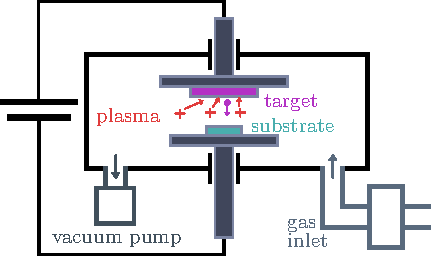
\includegraphics{../assets/sputtering.pdf}
	\caption{Schematic design of a sputtering chamber. \imcitetwo{jorrit}}
	\label{fig:sputtering}
\end{figure}

Sputtering is another \ac{pvd} technique. 
A target material is bombarded by energetic particles of a plasma or gas.
Microscopic particles of a solid material are ejected from its surface.
This leads to material evaporation and subsequent thin film growth. 

As energetic ions collide with atoms of the target material, 
an exchange of momentum sets off collision cascades in the target crystal system.
Eventually, the collision cascade reaches the target surface again. 
If the kinetic energy of the cascade surface atom is larger than the surface binding 
energy, the atom will be ejected.
The sputtered ions can originate from various sources: ion sources, radioactive material
or solar winds.

A schematic of a sputter chamber is depicted in \cref{fig:sputtering}.
The chamber is evacuated to create a vacuum environment, and a controlled background gas
is let into the chamber to regulate the deposition atmosphere and avoid unwanted 
chemical reactions.
A DC voltage is applied between the anode and cathode such that the cathode is 
negatively biased.
If the voltage is high enough (hundreds of kilovolts), the electrical field ionizes
the background gas and creates a plasma through glow discharge. 
The positive ions head towards the cathode and hit the target material.
Due to the sputtering process, the target material evaporates, the vapor distributes 
across the chamber and eventually condenses as a thin film on the substrate. 

\subsubsection{Thermal Evaporation}
Thermal evaporation is a subgroup of \ac{pvd} techniques. 
A target material is heated by electrical heating to temperatures near its boiling 
point.
The material begins to sublime and its vapor spreads through the chamber and condenses 
eventually on a substrate.
It is distinct from processes where the material vapor is altered after initial 
evaporation, like \ac{pld}. 

\subsubsection{Molecular Beam Epitaxy}
\begin{figure}
	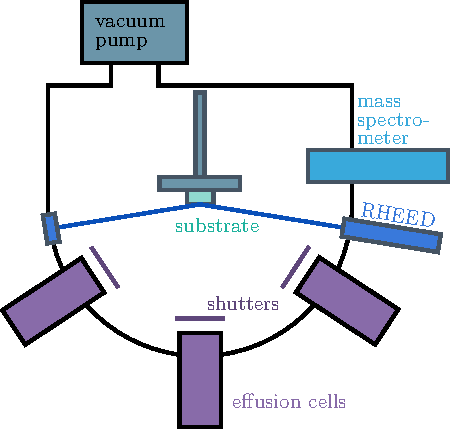
\includegraphics{../assets/mbe.pdf}
	\caption{Schematic design of a \ac{mbe} chamber. \imcitetwo{fernando}}
	\label{fig:mbe}
\end{figure}

\Ac{mbe} is a specialized technique of thermal evaporation used for epitaxial growth.
A schematic \ac{mbe} chamber is shown in \cref{fig:mbe}. 
One or more molecular or atomic beams from so-called Knudsen cells are directed towards 
a heated substrate.
The solid source materials are placed in evaporation cells.
Those evaporation cells provide an angular atomic or molecular distribution of the beam.
As with \ac{pld}, the substrate is heated and rotated for growth homogeneity.

A necessary condition to grow a sufficiently clean epilayer is ultra-high vacuum in the
order of \qtyrange{e-11}{e-14}{\bar} as well as ultrapure target materials.
Often the vacuum chamber walls are cryogenically screened to minimize flux of 
atoms from the chamber walls.
With that, it is possible to grow thin films with monolayer precision, just by opening 
and closing mechanical shutters of the beam sources. 
The ultra-high vacuum environment offers a reliable way to install in-situ measurement
instruments, such as a RHEED system or a mass spectrometer. 

Key element of a \ac{mbe} system are Knudsen cells. 
A typical Knudsen cell contains a crucible for the target, a temperature control system 
as well as a shutter. 
The Knudsen cell operates on the principle of effusion, where atoms or molecules escape 
through a small orifice. 
This results in a very precise way to control material flow. 

\subsubsection{Advantages compared to other Techniques}
The biggest advantage of a \ac{pld} system is its flexibility. 
It is a versatile technique for a wide range of thin film and multilayer applications.
Its material requirements are generally lower than those of \ac{mbe} or sputtering.
It often offers a stoichiometric transfer of multielement compounds from a single 
target to a substrate.
With that, it is possible to synthesize chemically complex materials. 
Especially oxide films can be easily controlled by background pressure. 

Another advantage of a \ac{pld} system is thin film fabrication time and cost. 
Compared to \ac{mbe}, \ac{pld} is less expensive, both in terms of initial investment 
and operational costs.
Most targets can be fabricated with simple lab equipment, for example ball mills and 
sintering furnaces, and commercially available powders.
Together with its high deposition rate, \ac{pld} is an excellent choice for
rapid prototyping.    

Reliable and user-friendly excimer lasers are already available. 
The laser operates independently of the deposition system, adhering to a separation 
of concerns design principle, which enhances modularity, simplifies system 
integration and troubleshooting.

\ac{pld} systems show an industrial upscaling potential. 
High mass deposition on large areas, with capabilities of covering up to an 8-inch 
diameter surface are already possible. 
Particularly excimer laser provide high pulse energy and a larger focus area at 
lower wavelengths, making them ideal for industrial-scale applications.

\ac{pld} also offers a wide parameter space, making it highly adaptable for various 
applications and offer tremendous optimization options.

\subsubsection{Drawbacks compared to other Techniques}
A major disadvantage of \ac{pld} is the trace element contamination of 
thin films due to the spatial expansion of the plasma plume as well as the use of 
multiple targets in one chamber.
Target constituents are located all within the chamber and can lead to permanent damage 
to the windows.
This is a crucial issue, especially for high-purity requirements.
Thin films fabricated by \ac{pld} (and sputtering) generally have a higher trace element contamination 
than thin films fabricated by \ac{mbe}. 

The process suffers from target preparation contamination too, as the target is 
prepared by mechanical ball mills, press molds and sintering ovens.
Source powders are only available with low purities which leads to additional 
contamination. 
Traces of construction alloy constituents are also present on the thin film. 

Another important disadvantage is droplet formation during the deposition process.
These droplets can be found in the deposited film and have a size of typically
\qty{1}{\micro \meter}.
This reduces the thin film quality tremendously.
Compared to \ac{mbe} or sputtering, \ac{pld} thin film quality and uniformity 
is inferior.  

To avoid droplet formation, velocity filters can be used.
A perpendicular arrangement of target and substrate is also applicable, because only
light plasma constituents are scattered perpendicular to the target.
Both methods reduce the deposition rate of the thin film and complicate the process 
as well.